\documentclass{article}
\usepackage[utf8]{inputenc}

\title{Maxout Networks}
\author{}
\date{}

\usepackage{natbib}
\usepackage{graphicx}
\usepackage{amsmath}
\usepackage[left=2.5cm,right=2.5cm,top=1cm,bottom=1.25cm]{geometry}
\usepackage{hyperref}
\usepackage{float}
\usepackage[export]{adjustbox}



\hypersetup{colorlinks=true,urlcolor=blue}
\pagenumbering{gobble}

\begin{document}

\maketitle

\section*{Link}
\href{https://arxiv.org/pdf/1302.4389}{arXiv} 

\section*{Summary}
\begin{itemize}
    \item The authors propose a new activation function that is designed to facilitate optimization by dropout and improves dropout's fast approximate model averaging technique.
    \item Dropout is similar to bagging where many different models are trained on different subsets of the data. Dropout training differs from bagging in that each model is trained for only one step and all of the models share parameters. Dropout is most effective when we use large learning rate. In this regime, each update can be seen as taking a significant update to a different model on a different subset of the training set.
    \item Maxout activation function takes maximum along the feature maps. If we have $k$ features, each of $m$ dimensions, we can take maximum along each feature maps to get $m$ outputs. A single maxout unit can be interpreted as making a piece wise linear approximation to an arbitrary convex function. Figure 1 shows how maxout function can implement the rectified linear, absolute value rectifier and approximate the quadratic activation function. 
    \begin{figure}[H]
        \centering
        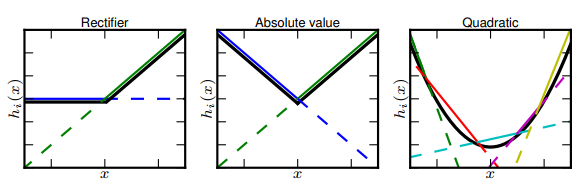
\includegraphics[scale=0.7]{maxout_approximation.png}
        \caption{Approximations using maxout}
        \label{fig:Figure 1}
    \end{figure}
    \item Maxout is a universal approximator that is, a maxout model with just two hidden units can approximate any continuous function provided that each individual unit has arbitrarily many affine components.
    \item Using maxout combined with dropout they were able to achieve state of the art performance on several benchmark dataset like MNIST, CIFAR-10, CIFAR-100 and SVHN.
    \item Rectified linear hidden unit followed by cross channel pooling does not perform as well as maxout unit. In particular rectified units do not gain benefit from cross channel pooling. They can match the performance of the maxout unit if filter is kept same(i.e., no cross channel pooling). So if a maxout unit has $k$ output from $k\times k$, the ReLU version will require us to use all $m\times k$ filters. This will increase output size for this layer and input and parameter size for the next layer by $k$ times.
    \item Multiplying layer weights by its probability of retaining during training $p$ does exact model averaging for a single layer, softmax regression. They argue that, dropout also does exact model averaging in deeper architectures provided that they are locally linear. Maxout can achieve this better than some activation functions with significant curvature like $tanh$ and thus performs much better than $tanh$ in the presence of dropout.   
    \item One important difference between dropout optimization and plain SGD is that dropout rapidly explores many different directions and rejects the ones that worsen the performance, while SGD moves slowly and steadily in the most promising direction.
    \item Dropout unit does not have the dying ReLU problem where a unit may become permanently inactive because it doesn't have a constant in its formulation like ReLU($max(x,0)$). Experiment shows that each maxout unit in the network was maximal for some training example, so all were utilised. 
    \item ReLU suffers from diminished gradient flow to the layers layer of the network in the presence of dropout. The variance of the gradient on the output weights was 1.4 times larger for maxout, while the variance on the gradient on the first layer weights was 3.4 times larger for maxout than rectifiers. 
\end{itemize}

\end{document}
